
\chapter{Introduction}
Power electronics systems, especially converters, lead to a more complex electrical field stress in insulation material of energy transmission systems as it introduces pulses (>1 kV) with high slew rates (>$10 \frac{kV}{\mu s}$) and high repetition frequencies (> 1 kHz) superimposed on low frequencies (50 Hz) or DC. The latter can cause enhanced partial discharges (PD) in the insulation system, i.e. a breakdown of a part of the insulation system. \cite{TransformerEngineering}. However, there are already effects below partial discharge inception that are not well understood, yet. They do as well result in an accelerated aging of the insulation due to the sustained application of the converter pulses. 
\newline

\begin{figure}[!ht]
  \begin{minipage}{0.5\textwidth}
  

  
  \centerline{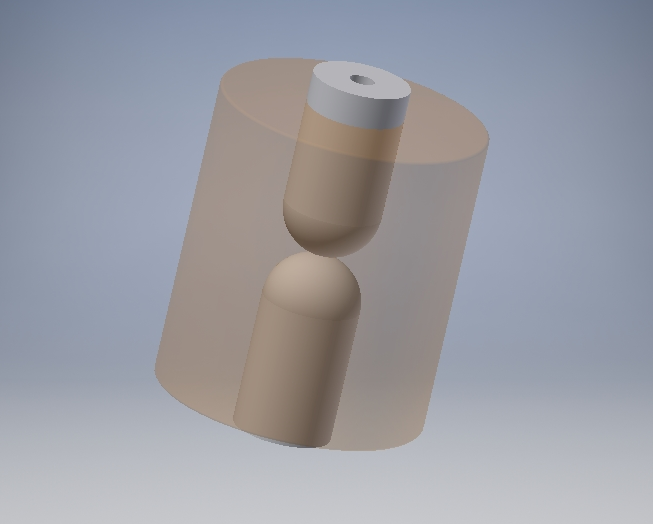
\includegraphics[height=0.2\textheight]{figures/intro/cad_epoxy}}
\caption{CAD model of epoxy specimen used for measurements}
	\label{fig.specimen}
	
	  \end{minipage}
	    \begin{minipage}{0.5\textwidth}
	  
  \centerline{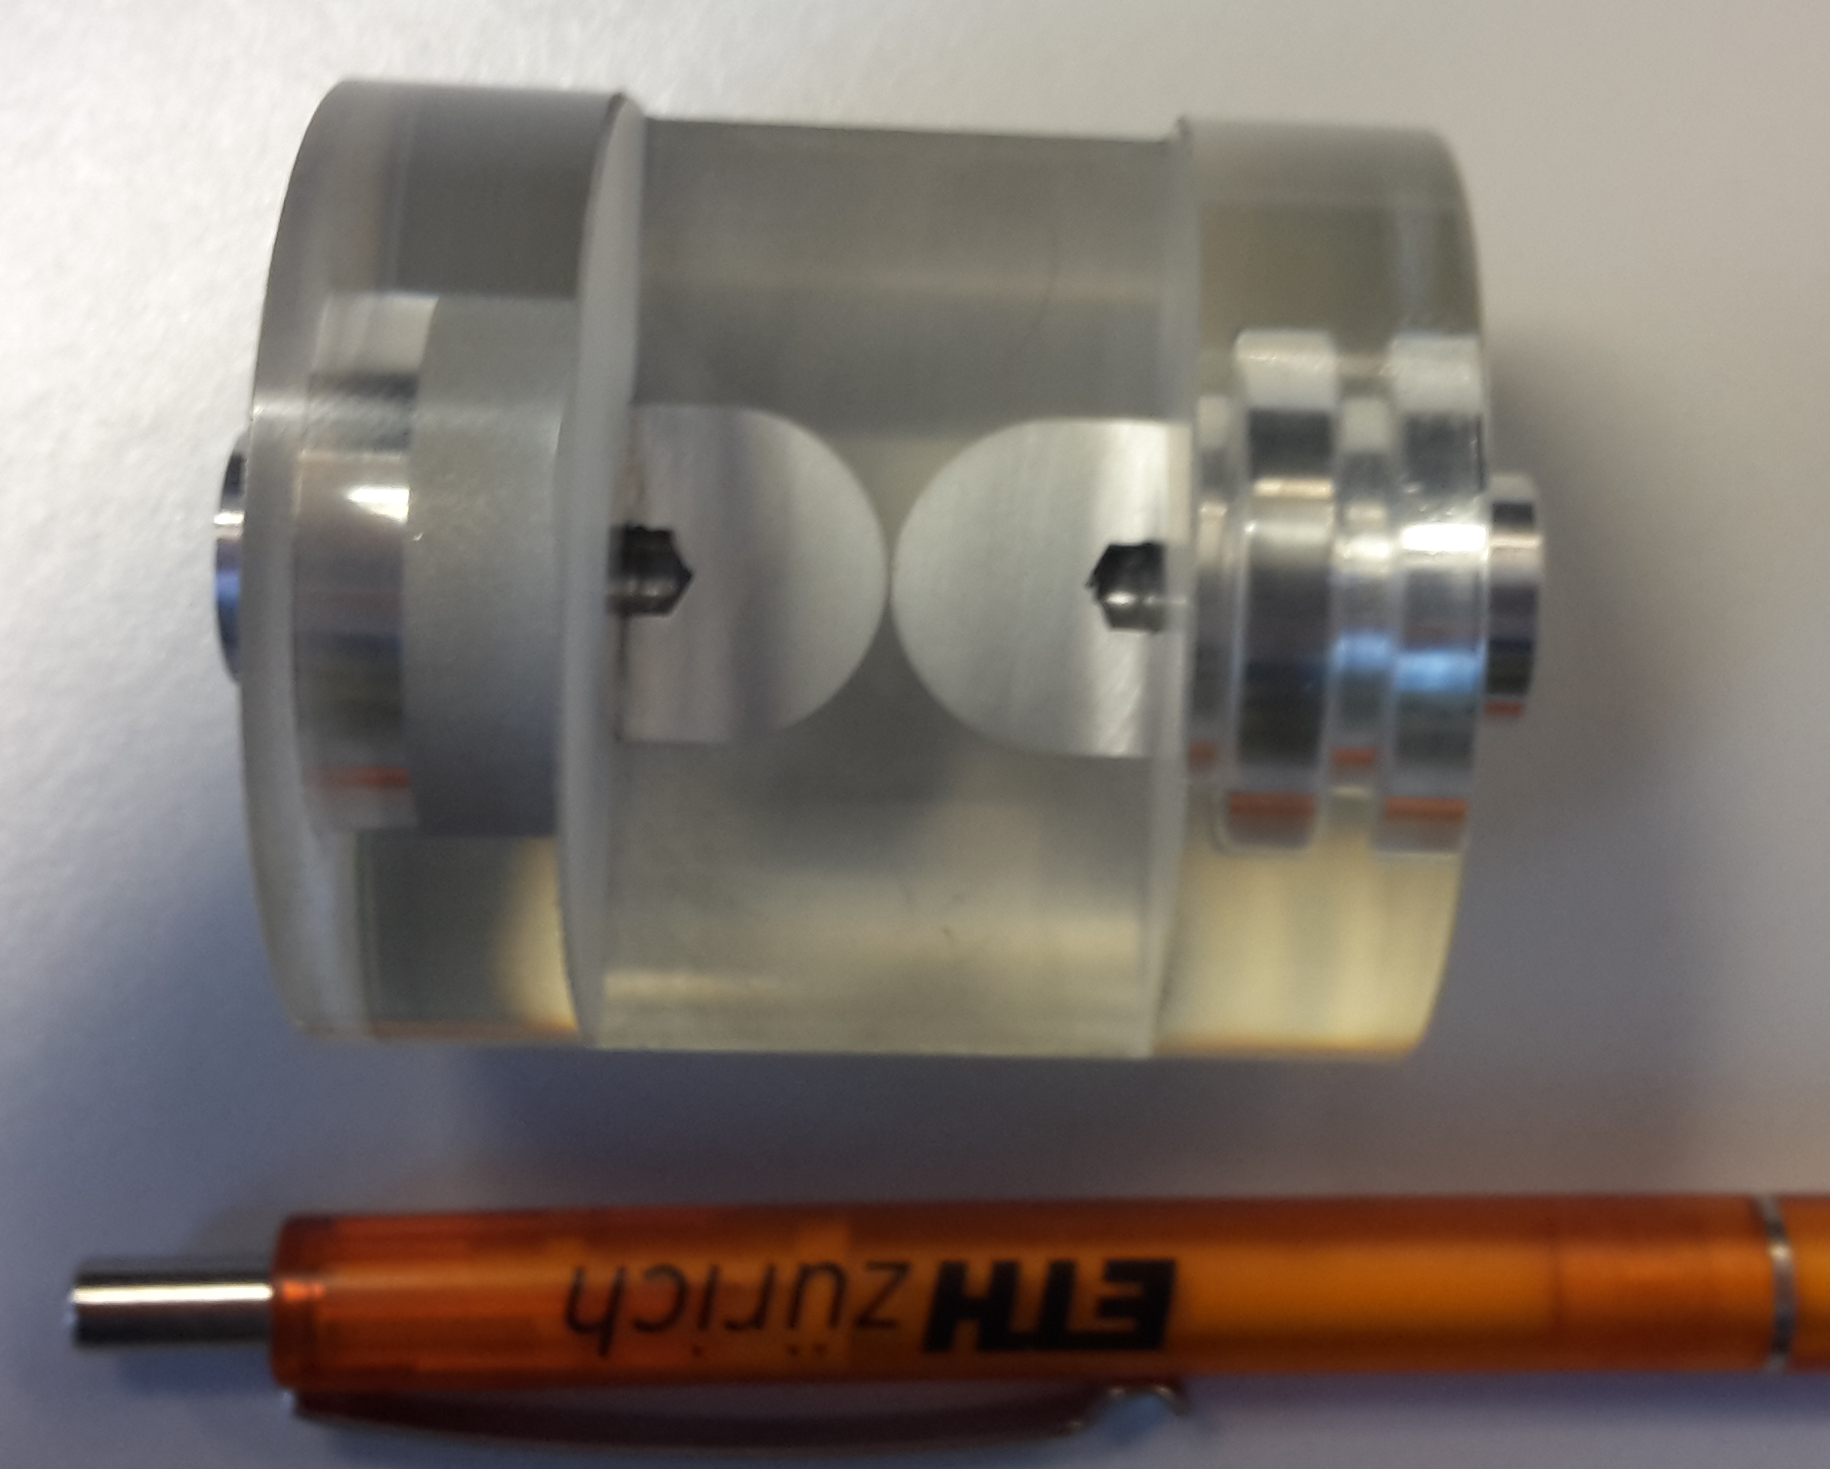
\includegraphics[height=0.2\textheight]{figures/intro/photo_epoxy2}}
\caption{Photo of Epoxy specimen used for measurements of the partial discharges. \protect\footnotemark}
	\label{fig.specimenphoto}
	  
	   \end{minipage}
\end{figure}
\footnotetext{{Both figures provided by Raphael F\"arber}}
In a new approach, a quantification of the pre-breakdown modification within the insulation material should be obtained with the use of an online monitoring of the dielectric permittivity for several harmonics of the applied pulse spectrum \cite{FaerberMVISS}.
The first part of this semester project is aimed at getting the dielectric permittivity by once measuring the capacity of the specimen shown in figure \ref{fig.specimen} in conjuction with numerical field simulations. When using a specimen after manufacturing it is assumed that it's dielectric permittivity is always the same. In order to be able to determine the distance of the two electrodes a reference measurement of the actual distance and the permittivity for two samples is made and a look-up table containing the electrode distance for different vacuum capacities is created. 

The second part of the project is the investigation of the suitability of current transformers in dielectric spectroscopy. With regard to the small capacitive current through the sample, it is the aim to prove or disprove that a current transformer does not deteriorate the signal in a way that makes dielectric spectroscopy is impossible. 


